\documentclass{article}
\usepackage{hyperref}
\usepackage[utf8x]{inputenc}
\usepackage[english,russian]{babel}
\usepackage{cmap}
\usepackage{amsmath}
\usepackage{graphicx}
\usepackage{amssymb}
\usepackage{indentfirst}
\graphicspath{ {./fig/} }
\usepackage[left=2cm,right=2cm,
    top=2cm,bottom=2cm,bindingoffset=0cm]{geometry}

\title{Билеты по линейной алгебре}

\begin{document}
\textbf{\centerline{Билеты по линейной алгебре для коллоквиума (by @zouyaia)}}
\tableofcontents
\newpage

\section{Отображения, композиция отображений. Образ и прообраз. Сюръекция, биекция, инъекция. Бином Ньютона и треугольник Паскаля.}

\textsc{Отображением $\varphi$} из множества $X$ в множество $Y$ называют соответствие, которое каждому
элементу $x \in X$ соотносит некоторый однозначно определённый элемент $y \in Y$:
$$\varphi:X\to Y\Leftrightarrow \forall x\in X \ \exists! y\in Y\colon y=\varphi(x).$$

При этом элемент $y\in Y$, соответствующий элементу $x\in X$, называют \textsc{образом} элемента $x$ при отображении $\varphi$.

При заданном $y\in Y$ совокупность всех $x\in X\colon \varphi(x)=y$, называют \textsc{прообразом} элемента $y$ и обозначают $\varphi^{-1}(y)$:
$$\varphi^{-1}(y)=\{x\in X\colon \varphi(x)=y\}$$

Если $f\colon X \to Y$ и $g\colon Y\to Z$, то отображение $\varphi\colon X\to Z$, заданное $\forall x\in X$ формулой $\varphi(x)=g(f(x))$,
называется \textsc{композицией (суперпозицией)} отображений $f$ и $g$, или сложной функцией, и обозначают $g\circ f$:
$$(g\circ f)(x)=g(f(x))$$

Отображение $\varphi\colon X \to Y$:
\begin{enumerate}
\item сюръективно, если $\forall y \in Y\ \exists x \in X\colon y = \varphi(x)$ – каждый элемент множества Y является прообразом хотя бы одного элемента множества X;
\item инъективно, если $\varphi(x)=\varphi(y)\Rightarrow x=y$ – разные элементы множества X переводятся в разные элементы множества Y;
\item биективно, если оно сюръективно и инъективно одновременно.
\end{enumerate}

\textsc{Бином Ньютона}
$$(a+b)^n = \sum^n_{k=0} C^k_n a^{n-k} b^k,$$
где $C^k_n = \frac{n!}{k!(n-k)!}$ - биноминальный коэффициент, $n,k \in \mathbb{N}, a,b \in \mathbb{R}$

\textsc{Треугольник Паскаля} – бесконечная треугольная таблица биномиальных коэффициентов. В этом треугольнике на вершине и по бокам стоят единицы. Каждое число равно сумме двух расположенных над ним чисел.

\centerline{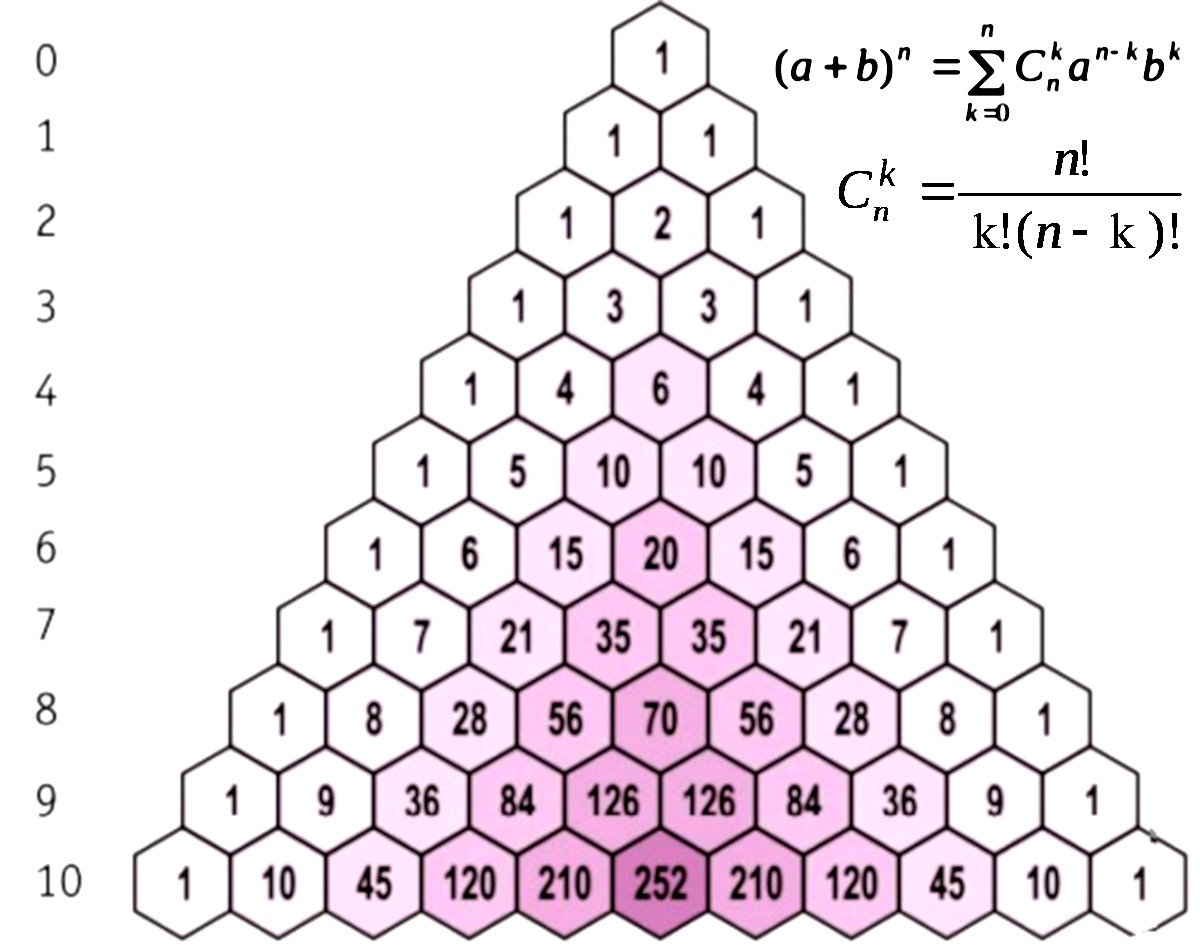
\includegraphics[width=0.5\linewidth]{tr_pascal.jpeg}}


\section{Основные алгебраические системы. Бинарная операция на множестве. Ассоциативность, коммутативность. Группоид, полугруппа, моноид, группа, абелева группа. Кольцо. Поле. Порядок группы/кольца/поля. Порядок элемента. Подгруппа, подкольцо, подполе. Идемпотенты и нильпотенты. Есть ли в поле делители нуля. Характеристика поля. Изоморфизм алгебраических систем.}

Пусть $M$ – произвольное множество. Операция $\circ$ называется \textsc{бинарной} операцией на $M$, если каждой паре элементов
$x,y\in M$ ставится в соответствие элемент $z\in M\colon x\circ y=z$ (свойство $\circ$ не выводить рез-тат из множества $M$ называется замкнутостью).

Тогда $<M, \circ>$ – \textsc{алгебраическая структура}.

\textsc{Группоид} – множество с одной бинарной операцией ($<M,\circ>$ - группоид).

Если $\forall a,b,c\in M$ выполняется $(a\circ b)\circ c=a\circ(b\circ c)$, то говорят что бинарная операция $\circ$ \textsc{ассоциативна}.
А алгебраическая структура $<M, \circ>$ является \textsc{полугруппой}.

Полугруппа называется \textsc{моноидом}, если $\forall a\in M \ \exists e\in M\colon a\circ e=e\circ a=a$, говорят что $e$ – нейтральный элемент.

Алгебраическая система $<G, \circ>$, состоящая из одной бинарной операции называется \textsc{группой}, если есть:
\begin{enumerate}
\item Ассоциативность
$$(a\circ b)\circ c=a\circ(b\circ c)$$
\item Нейтральный элемент
$$\forall a\in G \ \exists e\in G\colon a\circ e=e\circ a=a$$
\item Обратный элемент
$$\forall a\in G \ \exists b\in G\colon a\circ b=b\circ a=e$$
\end{enumerate}

Если $\forall a,b\in G$ имеет место $a\circ b=b\circ a$, то группа называется \textsc{абелевой (коммутативной)}.

Множество $R$ с двумя бинарными операциями называется \textsc{кольцом}, если на $R$ согласованно заданы два закона композиции $"+"$ и $"\cdot"$, так что выполняется:
\begin{enumerate}
    \item $\{ R, "+"\}$ – абелева группа,
    \item $\{ R, "\cdot"\}$ – полугруппа,
    \item Дистрибутивность: $a\cdot(b+c)=a\cdot b+a\cdot c, (b+c)\cdot a=b\cdot a+c\cdot a$
\end{enumerate}

Множество $K$ называется \textsc{полем}, если на $K$ согласованно заданы два закона композиции $"+"$ и $"\cdot"$, так что выполняется:
\begin{enumerate}
    \item $\{K, "+"\}$ – аддитивная абелева группа,
    \item $\{K, "\cdot"\}$ – мультипликативная абелева группа,
    \item Дистрибутивность: $a\cdot(b+c)=a\cdot b+a\cdot c, (b+c)\cdot a=b\cdot a+c\cdot a.$
\end{enumerate}

\textsc{Порядком {$|G|$} группы/кольца/поля {$G$}} называется число элементов в его носителе. 

\textsc{Порядок элемента {$g$}} из группы $G$ – это наименьший $n\in \mathbb{N}\colon g^n=e.$ Если такого $n$ нету, то $|g|=\infty$

Подмножество $L$ группы $G$ называется \textsc{подгруппой}, если:
\begin{enumerate}
    \item $L$ замкнута относительно бинарной операции $\circ$,
    \item $\forall a\in L\colon a^{-1}\in L$,
    \item $\exists e\in L\ \forall a\in L\colon a\circ a^{-1}=a^{-1}\circ a=e$.
\end{enumerate}

Подмножество $L$ кольца $R$ называется \textsc{подкольцом}, если:
\begin{enumerate}
    \item $L$ – подгруппа аддитивной группы кольца $R$,
    \item $L$ – замкнута относительно умножения.
\end{enumerate}

Подмножество $L$ поля $K$ называется \textsc{подполем}, если:
\begin{enumerate}
    \item $L$ – подкольцо кольца $K$,
    \item $\forall a\in L\ a\neq 0\Rightarrow a^{-1}\in L$,
    \item $1\in L$.
\end{enumerate}

Элемент $e\neq 0$ кольца $R$ называется \textsc{идемпотентом}, если $e^2=e$.

Элемент $x$ кольца $R$ называется \textsc{нильпотентом}, если $\exists n\in \mathbb{Z}\colon x^n=0$.

\textsc{Лемма} В поле нет делителей нуля

\textsc{Характеристика поля} — наименьшее положительное целое число $n$ такое, что сумма $n$ копий единицы равна нулю:
$n\cdot 1=0$.
Если такого числа не существует то характеристика равна 0 по определению. 

\textsc{Свойство:} характеристика поля всегда 0 или простое число ($char\ \mathbb{Q}=0$, $char\ \mathbb{Z}_p=p$).

Пусть ${\displaystyle G\!}$ и ${\displaystyle H\!}$ две алгебраические системы. Биекция ${\displaystyle f\colon G\to H}$ называется \textsc{изоморфизмом}, если для любых ${\forall a,b\in G\Rightarrow} \ {\displaystyle f(a)\cdot f(b)=f(a\cdot b).}$

\section{Отношение эквивалентности. Фактормножество. Эквивалентность, согласованная с операциями. Кольцо вычетов Z. Арифметика в кольце вычетов. Когда кольцо вычетов является полем. Бином Ньютона в поле Z. Малая теорема Ферма. Линии на плоскости.}
Отношение $R$ называется \textsc{отношением эквивалентности}, если выполняется:
\begin{enumerate}
    \item Рефлексивность: $a\sim a$
    \item Симметричность: $a\sim b\Rightarrow b\sim a$
    \item Транзитивность: $a\sim b$ и $b\sim c\Rightarrow a\sim c$
\end{enumerate}

\textsc{Фактормножество} по отношению $R$ – множество, состоящее из всех классов эквивалентности.

Отношение эквивалентности $R$ на множестве $M$ называется \textsc{согласованным с операцией} *, если:
$$a\sim a', b\sim b' \Rightarrow a*b\sim a'*b'.$$

\textsc{Классом вычетов} числа $a$ по модулю $n$ называется такое множество:
$$[a]_n=\{b\in \mathbb{Z}|(a-b)\vdots n\}.$$

\textsc{Арифметика в классе вычетов:}
$a_1\equiv b_1 (mod\ n)$ и $a_2\equiv b_2 (mod\ n)\Rightarrow$
\begin{enumerate}
    \item $a_1+a_2\equiv b_1+b_2 (mod\ n)$
    \item $a_1a_2\equiv b_1b_2 (mod\ n)$
\end{enumerate}

\textsc{Кольцом вычетов} $Z_n$ называется множество всех классов вычетов по модулю $n$ (фактормножество):
$$Z_n=\{[0]_n, [1]_n,\dots , [n-1]_n\}$$

\textsc{Арифметика в кольце вычетов:}
\begin{enumerate}
    \item $[a]_n+[b]_n=[a+b]_n$
    \item $[a]_n\cdot [b]_n=[ab]_n$
\end{enumerate}

\textsc{Теорема} Кольцо вычетов $Z_n$ является полем тогда и только тогда, когда $n$ – простое число:

\textsc{Бином Ньютона $(a+b)^p$ в поле $\mathbb{Z}_p$}
$$(a+b)^p=a^p+b^p$$
$$0<k<p\Rightarrow C^k_p=\frac{p!}{k!(p-k)!}=\frac{(p-k+1)\dots(p-1)p}{k!}\vdots p=0$$

\textsc{Малая т.Ферма}
$$a^p\equiv a\ (mod\ p), p\in P, a\in Z$$

\textsc{Линии на плоскости $\mathbb{Z}^2_p$}
\begin{enumerate}
    \item Через любые две точки проходит одна и только одна прямая
    \item Для каждой прямой и не принадлежащей ей точки существует ровно одна прямая, не пересекающаяся с данной
    \item Существует три точки, не лежащие на одной прямой
\end{enumerate}
Прямая – множество точек (x, y), удовлетворяющих уравнению $ax+by=c$, где хотя бы один из коэффициентов отличен от 0. 

\section{Группа подстановок: проверка аксиом, разложение на циклы, на транспозиции, декремент и четность подстановки, четность произведения, подгруппа четных подстановок.}
Биективное преобразование $\sigma$ непустого множества M называется \textsc{подстановкой} множества M.

Множество $S(M)$ всех подстановок непустого мн-ва $M$ образует группу относительно бинарной операции композиции $<S(M),\circ>$:
\begin{enumerate}
    \item Ассоциативность: $f\colon X\to Y, g\colon Y\to U, h\colon U\to V\colon (h\circ (g\circ f))(x)=h(g(f(x)))=(h\circ g)\circ f(x)$
    \item Нейтральный: $\varepsilon(x)=x$
    \item Обратный: $\sigma(x)=y\Rightarrow \sigma^{-1}(y)=x$
\end{enumerate}

Подстановку $\sigma$ называют \textsc{циклом} длины $s$, если множество ее перемещаемых символом $T_\sigma$ можно занумеровать так: $T_\sigma=\{i_1,i_2,\dots ,i_s\}$, при чем $\sigma(i_1)=i_2,\dots,\sigma(i_s)=i_1$.

Пусть $\sigma$ не тождественная подстановка из $S(M)$, тогда $\sigma$ можно представить в виде \textsc{произведения попарно независимых циклов}, это разложение единственно с точностью до порядка сомножителей.

Цикл длины 2 называется \textsc{транспозицией}.
Всякую подстановку $\sigma$ из $S(M)$ можно разложить на $n-s$ транспозиций, где $s$ – число независимых циклов, $n$ – число символов.

\textsc{Декремент} подстановки $d(\sigma)=n-s$.

\textsc{Знак} подстановки $sgn(\sigma)=(-1)^{d(\sigma)}$.
Если $sgn(\sigma)=1$, то подстановка \textsc{чётная}, если же $sgn(\sigma)=-1$ – нечётная.

Умножение на транспозицию меняет знак подстановки на противоположный:
$d(\sigma\tau)=d(\sigma)\pm 1$

\textsc{Знак произведения} подстановок равен произведению знаков:
$sgn(\sigma\pi)=sgn\sigma \cdot sgn\pi$

\textsc{Теорема Кэли:} любая конечная группа G порядка n изоморфна некоторой подгруппе группы S(M)

\section{Арифметика матриц: сложение, умножение, транспонирование. Кольцо квад- ратных матриц над полем. Перестановочные матрицы. Разложение квадратной мат- рицы в произведение диагональной и трансвекций. Блочные матрицы.}

\textsc{Сложение матриц на {<$S, +, \cdot$>}} $A=(a_{i,j})_{m\times n}, B=(b_{i,j})_{m\times n}$
$$A+B=(a_{i,j}+b_{i,j})_{m\times n}$$

\textsc{Умножение матриц на {<$S, +, \cdot$>}} $A=(a_{i,j})_{m\times s}, B=(b_{i,j})_{s\times n}$
$$A\cdot B=(c_{i,j})_{m\times n}$$
$$c_{i,j}=\sum_{k=1}^{s} a_{ik}b_{kj}$$

\textsc{Транспонирование $A^T$}
$$A=(a_{ij})_{m\times n}\Rightarrow A^T=(a_{ji})_{n\times m}$$

Пусть $<R, +, \cdot>$ – поле, а $n\in \mathbb{N}$. Тогда квадартные матрицы $M_n(R)$ образуют кольцо относительно оп-ций +, $\cdot$ над полем R.

Матрицы А и B называют \textsc{перестановочными}, если $AB=BA$

\textsc{Теорема.} Пусть есть матрица $A\in M_n(F)$. Тогда найдутся такие трансвекции $T_1,T_2,\dots,T_k,\dots,T_s$ и диагональная матрица 
$D\in M_n(F),$ что $A=T_1T_2\dots T_kDT_{k+1}\dots T_s$

\textsc{Блочная матрица} – матрица, разделенная горизонтальными и вертикальными линиями на блоки, которые представляют собой подматрицы.

\section{Определители квадратных матриц и их свойства. Обратная матрица. Теорема Крамера. След квадратной матрицы и его свойства.}
Определитель квадратной матрицы – это число, определяющее некоторые свойства матрицы.

\textsc{Свойства определителя (для строк):}
\begin{enumerate}
    \item При умножении некоторой строки матрицы на число, определитель умножается на это число;
    \item Если одна из строк нулевая, то $det A=0$
    \item $A\in M_n(F), \lambda \in F \ det(\lambda\cdot A)=\lambda^ndet A$
    \item Если матрица A отличается от B тк r-ой строкой, то для матрицы C, получающейся сложением r-ых строк этих матриц, выполняется: $det C=det A+det B$
    \item Если в матрице две строки совпадают, то ее определитель равен 0
    \item При перестановке местами двух строк матрицы, ее определитель меняет знак
    \item При добавлении к строке матрицы другой строки, умноженной на число, определитель не меняется
    \item Определитель треугольной матрицы равен произведению эл-ов на главной диагонали
    \item $det A^T=det A$
    \item $det(AB)=det A\cdot det B$
\end{enumerate}
Если в каждом утвержденнии о св-вах определителя применить то же самое к столбцам матрицы, то утверждения останутся верными

\textsc{Теорема Крамера} Если матрица A не вырожденная, то система $A\cdot x=B$ имеет единственное решение,
которое может быть найдено по формуле Крамера: $x_i=\frac{det A_i}{det A}$, где $A_i$ – матрицы получающиеся заменой i-ого столбца на столбец b

\textsc{Обратная матрица}
$$A^{-1}=\frac{1}{det A}\cdot \hat{A}^T,$$
где $\hat{A}^T$ – союзная матрица, составленная из алгебраических дополнений для соответствующих элементов транспонированной матрицы.

\textsc{Следом} квадратной матрицы называют сумму ее элементов, стоящих на главной диагонали.
Свойства следа:
\begin{enumerate}
    \item $tr(A+B)=trA+trB$
    \item $trA^T=trA$
    \item $tr(AB)=tr(BA)$
\end{enumerate}

\section{Поле комплексных чисел C: определение, единственность, существование, геометрическое описание сложения и умножения, формула Муавра, извлечение корней, первообразные корни из 1.}

\textsc{Аксиомы (определение) поля комплексных чисел $\mathbb{C}$:}
\begin{enumerate}
    \item Содержит подполе, изоморфное $\mathbb{R}$
    \item Содержит элемент $i: i^2=-1$
    \item Минимальное среди полей, удовлетворяющих 1. и 2.
\end{enumerate}

Поле комплексных чисел \textsc{существует и единственно} с точностью до изоморфизма

Алгебраическая форма: $z=a+bi$, где $Re(z)=a$ – вещественная часть, а $Im(z)=b$ – мнимая часть.

\textsc{геометрический смысл сложения $\mathbb{C}$.}
На плоскости, где каждое комплексное число  отображено как вектор, идущий от начала коодинат 0 до точки, сложение комплексных чисел сводится к сложению соответствующих векторов по правилу параллелограмма.

\textsc{геометрический смысл умножения $\mathbb{C}$.}
Поворот и растяжение, т.к. $z_1z_2=r_1r_2(\cos{\varphi_1+\varphi_2}+i\sin{\varphi_1+\varphi_2})$

\textsc{Формула Муавра}
$$z^n=(r(\cos\varphi+i\sin\varphi))^n=r^n(\cos n\varphi+i\sin n\varphi)$$
Извлечение корней из комплексного числа также выполняется по формуле Муавра ($\sqrt[n]{z}=z^{\frac{1}{n}}$)

\textsc{Первообразные корни из 1}
$$\varepsilon_k=\cos\frac{2\pi k}{n}+i\sin\frac{2\pi k}{n}$$
$$\mathbb{C}_n=\{\varepsilon_k|k=0,\dots,n-1\}$$
Корень называется \textsc{первообразным}, если все остальные корни представимы в виде его степени

\section{Кольцо многочленов над полем. Делимость в кольце многочленов, алгоритм Евклида. НОД многочленов. Схема Горнера. Приводимые и неприводимые многочлены. Аналог основной теоремы арифметики. Алгебраически замкнутые поля. Основная теорема алгебры. Теорема Виета. Построение конечных полей.}
Многочлен f от переменной x над полем F
$$f(x)=a_nx^n+a_{n-1}x^{n-1}+\dots+a_1x+a_0=\sum^n_{k=0}a_kx^k, a_k\in F,$$
$a_n\neq 0$ – старший коэффициент, сам индекс n – степень многочлена f, обозн $deg\ f=n$

$F[x]$ – все многочлены над полем F; $f=g$ два многочлена равны, когда раыны их коэффициенты при соответствующих степенях

Операции над кольцом многочленов $<F[x], +, \cdot>$, $f,g\in F[x]$:
\begin{enumerate}
    \item Сумма: $$f+g=\sum_{k=0}(a_k+b_k)x^k$$
    \item Произведение: $$f\cdot g=\sum_{i+j=k}a_ib_jx^k$$
\end{enumerate}

Свойства степени многочлена: 1. $deg (f+g)\leq \max(deg\ f, deg\ g)$ 2. $deg (fg)\leq deg\ f+deg\ g$

\textsc{Делимость в кольце многочленов}

Теорема 
$$f, g\in F[x], g\neq 0\Rightarrow\exists q, r\in F[x]\colon f=gq+r,$$
где многочлены q(неполное частное), r(остаток) определены однозначно, причем $deg\ r<deg\ g$.

Свойства делимости в кольце многочленов:
\begin{enumerate}
    \item $g\mid f, g\mid h \Rightarrow g\mid (f+h)$
    \item $g\mid f\Rightarrow \forall h\in F[x]\ g\mid (hf)$
    \item $deg\ g=0\Rightarrow \forall f\in F[x]\ g\mid f$
    \item $deg\ h=0,\ g\mid f\Rightarrow (gh)\mid f$
\end{enumerate}

Т. Безу Остаток от деления многочлена f на двучлен (x-c) равен значению многочлена в точке c.

\textsc{Схема Горнера}
$$f=a_nx^n+a_{n-1}x^{n-1}+\dots+a_1x+a_0$$
$$f(x)=(x-c)(b_{n-1}x^{n-1}+b_{n-2}x^{n-2}+\dots+b_1x+b_0)+r$$
\begin{equation*}
    \begin{cases}
        x^n: a_n=b_{n-1} \\
        x^{n-1}: a_{n-1}=b_{n-2}-cb_{n-1} \\
        \dots \\
        x^1: a_1=b_0-cb_1 \\
        x^0: a_0=r-cb_0
    \end{cases}
\end{equation*}
\begin{equation*}
    \begin{cases}
        b_{n-1}=a_n \\
        b_{n-2}=a_{n-1}+cb_{n-1} \\
        \dots \\
        b_0=a_1+cb_1 \\
        r=a_0+cb_0
    \end{cases}
\end{equation*}

\centerline{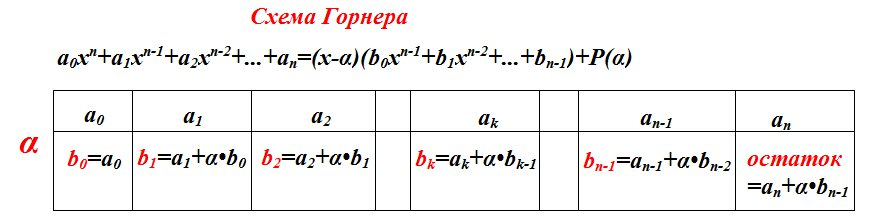
\includegraphics[width=0.7\linewidth]{gr62.jpeg}}

\textsc{Алгоритм Евклида}
Пусть r – остаток от деления f на g. Тогда мн-во общих делителей f и g совпадает с мн-вом общих делителей g и r. В частности совпадает их НОД $d=(f,g)=(g,r)$.

Т. (Линейное представление НОД) $f, g\in F[x], g\neq 0\Rightarrow\exists d=(f,g)\colon d=fu+gv,\ u,v\in F[x]$. Более того $deg(f), deg(g)>0\Rightarrow deg\ u<deg\ g, deg\ v<deg\ f$

\textsc{Приводимые и неприводимые многочлены}
Многочлен $f\in F[x], deg\ f>0$ называется неприводимым над F, если из его разложения на произведение многочленов $f=u\cdot v\Rightarrow deg\ u=0$ или $deg\ v=0$ ($\forall u,v\in F[x]$).

\textsc{Аналог основной теоремы арифметики}
Т. $f\in F[x], f\neq 0\Rightarrow\exists\alpha\in F$ – скаляр над полем F, и $\exists p_1,p_2,\dots,p_r$ – неприводимые многочлены со старшим коэф-ом 1. Тогда f раскладывается на произвдение скаляра и многочленов и такое разложение единственно:
$$f=\alpha p_1p_2\dots p_r$$

Поле F называется \textsc{алгебраически замкнутым}, если каждый многочлен ненулевой степени с коэф. из F[x] имеет в этом поле корень.

\textsc{основная теорема алгебры}
Поле $\mathbb{C}$ алгебраически замкнуто.

\textsc{Теорема Виета}
$$f(x)=a_nx^n+a_{n-1}x^{n-1}+\dots+a_1x+a_0$$
$$f(x)=a_n(x-c_1)(x-c_2)\dots(x-c_n)=$$
$$=a_n(x^n+x^{n-1}(-c_1-\dots-c_n)+x^{n-2}(c_1c_2+\dots+c_{n-1}c_n)+\dots+(-1)^nc_1c_2\dots c_n)$$

\begin{equation*}
    \begin{cases}
        c_1+c_2+\dots+c_n=-\frac{a_{n-1}}{a_n} \\
        c_1c_2+c_1c_3+\dots+c_{n-1}c_n=\frac{a_{n-2}}{a_n} \\
        \dots \\
        c_1c_2\dots c_n=(-1)^n\frac{a_0}{a_n}
    \end{cases}
\end{equation*}
Сумма корней квадратного уравнения $ax^2+bx+c=0$, где $a \neq 0$, равна $-\frac{{b}}{{a}}$, а произведение корней равно $\frac{{c}}{{a}}$.

\textsc{Построение конечных полей.}
Используя неприводимые многочлены, можно строить новые конечные поля – расширения простых полей $F_p$:
1. Выбираем простое p и фиксируем поле $F_p=<\{0,1,\dots,p-1\},+,\cdot>$ 2. Рассматриваем кольцо многочленов $F_p[x]$ над ним
3. Выбираем натуральное n и неприводимый многочлен $P(x)=a_nx^n+\dots+a_1x+a_0\in F_p[x]$ 4. $f(x)=Q(x)\cdot P(x)+R(x)$, R(x) - конечное поле Галуа.

\section{Многочлены с рациональными коэффициентами. Лемма Гаусса. Признак Эйзенштейна.}

$a_i\in \mathbb{Q}, f(x)\in Q[x]$

Т. Если $f(x)\in \mathbb{Z}$ и этот многочлен имеет рациональный корень $\frac{u}{v}$, НОД(u,v)=1, тогда u – делитель
свободного коэф-та $u\mid a_0$, а v – делитель старшего коэф-та $v\mid a_n$. Кроме того $u-mv\mid f(m),\ \forall m\in \mathbb{Z}$

\textsc{Лемма Гаусса}
Если многочлен с челыми коэффициентами раскладывается в произведение двух многочленов с рациональными коэффициентами, то он раскладывается в произведение пропорциональных им многочленов с целыми коэффициентами.

\textsc{Признак Эйзенштейна}
$$f(x)=a_nx^n+a_{n-1}x^{n-1}+\dots+a_1x+a_0, a_i\in \mathbb{Z}[x]$$
Если $\exists p\in P$, такое что
\begin{enumerate}
    \item $p\mid a_k\ \forall k=0,1,\dots,n-1$
    \item $p\nmid a_n$
    \item $p^2\nmid a_0$
\end{enumerate}
То многочлен f неприводим над $\mathbb{Q}$

\section{Векторные (линейные) пространства. Аксиомы векторного пространства и следствия из них. Алгебры. Подпространства и подалгебры. Тело. Теорема Веддербёрна.}

\textsf{Векторное пространство V над полем F – множество векторов с бинарной операцией + (сложения) и унарной операцией $v\to\alpha v$ (умножения на скаляр) для любого $\alpha\in F$}

Аксиомы векторного пространства:
\begin{enumerate}
    \item $<V, +>$ – абелева группа
    \item $\forall\alpha\in F, \forall u,v\in V\ \ \alpha(u+v)=\alpha u+\alpha v$
    \item $\forall\alpha,\beta\in F, \forall u\in V\ \ (\alpha+\beta)u=\alpha u+\beta u$
    \item $\forall\alpha,\beta\in F, \forall u\in V\ \ (\alpha\beta)u=\alpha(\beta u)$
    \item $\forall u\in V\ \ 1u=u$
\end{enumerate}

Следствия из аксиом:
1. $\alpha 0=0\ \ $
2. $\alpha (-v)=-\alpha v\ \ $
3. $\alpha(u-v)=\alpha u-\alpha v\ \ $
4. $0v=0, 0\in V\ \ $
5. $(-1)v=-v\ \ $
6. $(\alpha-\beta)u=\alpha u-\beta u$

\textsf{Алгебра} над полем F – множество с двумя бинарными операциями + и $\cdot$, унарной операцией умножения на скаляр $a\to\alpha a$ ($\forall\alpha\in F$)
\begin{enumerate}
    \item A – кольцо относительно +, $\cdot$
    \item A – векторное пространство относительно +, умножения на скаляр
    \item $\forall\alpha\in F\ \ \forall a,b\in A\ \ \alpha(ab)=(\alpha a)b=a(\alpha b)$
\end{enumerate}

Векторное пространство $U\neq \varnothing$ над F называется \textsf{подпространством} пр-ва V ($U\subseteq V$), если U замкнуто относительно операций, заданных на V:
$$\forall u,v\in U\Rightarrow u+v\in U, \alpha v\in U, \alpha u\in U$$

Аналогично определяется и \textsf{подалгебра}:
алгебра $A'\neq \varnothing$ над F называется \textsf{подалгеброй} алгебры A ($A'\subseteq A$), если A' замкнута относительно операций, заданных на A:
$$\forall a,b\in A'\Rightarrow a+b\in A', a\cdot b\in A', \alpha a\in A', \alpha b\in A'$$

\textsf{Тело} – ассоциативное кольцо с 1, в которой каждый ненулевой элемент обратим.
Если умножение коммутативно, тело превращается в поле. (пример тела: множество кватернионов)

\textsf{Т. Веддербёрна:} всякое конечное тело является полем.

\section{Линейная (не)зависимость систем векторов и свойства линейно (не)зависимых систем. Линейная оболочка системы векторов.}

Система векторов – множество повторяющихся занумерованных векторов: $A = \{a_1,a_2,\dots,a_n\}$. Линейная комбинация системы векторов:
$$\lambda_1a_1+\lambda_2a_2+\dots+\lambda_na_n,$$
где $\lambda_i\in F$ – коэффициенты лин. комбинации, $a_i\in V$ – вектора.

Система векторов A называется \textsf{линейно независимой}, если
$$\lambda_1a_1+\dots+\lambda_na_n=0\Rightarrow \lambda_1=\dots=\lambda_n=0,$$
то есть из равенства лин. комбинации 0 следует ее тривиальность – равенство всех коэффициентов 0.

Говорят, что вектор a \textsf{линейно выражается} через систему A, если существует лин. комбинация равная a.
$$a=\lambda_1a_1+\lambda_2a_2+\dots+\lambda_na_n$$

\textsf{Лемма 1}
Система векторов является \textsf{линейно зависимой} тогда и только тогда, когда в ней найдется вектор, который линейно выражается через остальные.

Свойства линейно зависимых и независимых систем:
\begin{enumerate}
    \item Если в систему векторов входит нулевой вектор, то она линейно зависима
    \item Если в системе векторов имеется два равных или противоположных вектора, то она линейно зависима.
    \item Если в системе векторов имеется два пропорциональных вектора $\vec{a}_i=\lambda\vec{a}_j$, то она линейно зависима.
    \item Система из $k>1$ векторов линейно зависима тогда и только тогда, когда хотя бы один из векторов есть линейная комбинация остальных.
    \item Любые векторы, входящие в линейно независимую систему, образуют линейно независимую подсистему.
    \item Система векторов, содержащая линейно зависимую подсистему, линейно зависима.
    \item Если система векторов $\vec{a}_1,\vec{a}_2, \ldots, \vec{a}_k$ линейно независима, а после присоединения к ней вектора $\vec{a}$ оказывается линейно зависимой, то вектор $\vec{a}$ можно разложить по векторам $\vec{a}_1,\vec{a}_2,\ldots,\vec{a}_k$, и притом единственным образом, т.е. коэффициенты разложения находятся однозначно.
\end{enumerate}

\textsf{Линейной оболочкой L} системы векторов $A = \{a_1,a_2,\dots,a_n\}$ называется мн-во линейных комбинаций этих векторов (результатов этих комбинаций):
$$L(A)=<A>=<a_1,a_2,\dots,a_n>=\{\lambda_1a_1+\dots+\lambda_na_n | \lambda_i\in F, a_i\in A\}$$

\section{Метод Гаусса. Классификация СЛАУ (определённые, неопределённые, совместные, несовместные). Структура решения СЛАУ. Метод Гаусса на языке умножения матриц.}

\textsf{Метод Гаусса} — классический метод решения системы линейных алгебраических уравнений (СЛАУ) путем последовательного исключения переменных, когда с помощью элементарных преобразований система уравнений приводится к равносильной системе треугольного (ступенчатого) вида, из которой последовательно, начиная с последних (по номеру), находятся все переменные системы.

СЛАУ называется (классификация):
\begin{enumerate}
    \item совместной, если имеет хотя бы одно решение
    \begin{enumerate}
        \item определённой, если ровно одно решение
        \item неопределённой, если более одного решения
    \end{enumerate}
    \item несовместной, если она не имеет ни одного решения
\end{enumerate}

\textsf{Структура решения СЛАУ.} Общее решение неоднородной СЛАУ есть сумма общего решения однородной и частного решения неоднородной:
$$X_{on}=X_{oo}+X_{hn}$$


\textsf{Метод Гаусса для умножения матриц} – последовательное умножение матриц на элементарные:
\begin{enumerate}
    \item меняем ур-я местами, строчки i, j меняем местами ($P_{ij}$)
    \item умножение на $\alpha\in F, (Q_i(\alpha))$ 
    \item к i ур-ю прибавляем j ($T_{ij}(\alpha)$)
\end{enumerate}

\section{Основная лемма о линейной зависимости. Базис и размерность векторного пространства. Описание конечномерных пространств с точностью до изоморфизма. Теорема о размерности пространства решений однородной СЛАУ. Базис пространства решений однородной СЛАУ — ФСР.}

\textsf{Основная лемма о линейной зависимости}
Если $b_1,b_2,\dots,b_m$ линейно выражаются через $a_1,a_2,\dots,a_n\in V \Rightarrow b_1,b_2,\dots,b_m$ – линейно зависимы (m>n).

\textsf{Базисом} векторного пространства называется всякое максимальное линейно независимое множество векторов из этого пространства.

Число векторов n в базисе ненулевого векторного пространства V называется \textsf{размерностью} этого пространства (dim\ V=n).

\textsf{Конечномерное пространство} – векторное пространство, в котором имеется базис.

Т1. $A\subset V$, где A – конечномерное векторное пространство, V – бесконечномерное векторное пространство.

Т2. Все базисы конечномерного векторного пространства содержат одинаковое число векторов.

Т3. Всякую линейно независимую систему векторов конечномерного векторного пространства можно дополнить до базиса.

Т4. Всякое подпространство конечномерного векторного пространства тоже конечномерно.

Т5. Векторное пространство V размерности dim V=n над полем F изоморфно пр-ву столбцов $F^n$

\textsf{Т. о размерности пр-ва решений однородной СЛАУ.} Размерность пространства решений системы линейных однородных уравнений равна $n-r$, где n – число неизвестных, r – ранг матрицы системы.

Базис пространства решений однородной СЛАУ называется её фундаментальной системой решений(ФСР).

\section{Переход от одного базиса к другому. Матрица перехода и её свойства.}

Очевидно, что в одном и том же векторном пространстве можно выбрать множество базисов. Пусть в V выбрано два базиса $A=(a_1,a_2,\dots,a_n)$ и $B=(b_1,b_2,\dots,b_n)$.

Векторы базиса B могут быть выражены через векторы базиса A:
\begin{equation*}
    \begin{cases}
        b_1=t_{11}a_1+t_{21}a_2+\dots+t_{n1}a_n \\
        b_2=t_{12}a_1+t_{22}a_2+\dots+t_{n2}a_n \\
        \dots \\
        b_n=t_{1n}a_1+t_{2n}a_2+\dots+t_{nn}a_n \\
    \end{cases}
\end{equation*}
Из коэффициентов разложения можно составить матрицу $$T=
\begin{pmatrix}
    t_{11} & t_{12} & \dots & t_{1n} \\
    t_{21} & t_{22} & \dots & t_{2n} \\
    \dots & \dots & \dots & \dots \\
    t_{n1} & t_{n2} & \dots & t_{nn}
\end{pmatrix}
$$
Матрица называется \textsf{матрицей перехода} от базиса A к базису B. В ее столбцах записаны координаты векторов $(b_1,b_2,\dots,b_n)$ относительно базиса A.
$$(b_1,b_2,\dots,b_n)=(a_1,a_2,\dots,a_n)T=(a_1,a_2,\dots,a_n)(A\rightsquigarrow B)$$

Свойства матрицы перехода:
\begin{enumerate}
    \item $(A\rightsquigarrow A)=E$
    \item $(A\rightsquigarrow B)(B\rightsquigarrow C)=(A\rightsquigarrow C)$
    \item $(A\rightsquigarrow B)(B\rightsquigarrow A)=E$
\end{enumerate}

\section{Ранг и база системы векторов. Ранг матрицы, теорема о ранге матрицы (= теорема о базисном миноре). Лемма о вычислении ранга матрицы. Теорема Кронекера-Капелли.}
\textsf{База} системы векторов – это эквивалентная ей линейно независимая подсистема.

\textsf{Ранг} системы векторов – число векторов в базе.

Строчный (Столбцовый) ранг матрицы – размерность линейной оболочки системы её строк (столбцов). Минор r-ого порядка – определитель подматрицы при выделении $r$ строк и $r$ столбцов.

Т. Столбцовый, строчный и минорные ранги совпадают.

\textsf{Ранг матрицы} — наивысший из порядков всевозможных ненулевых миноров этой матрицы.

\textsf{Теорема о базисном миноре:} строки (столбцы), пересекающие базисный минор линейно независимы. Любая строка (столбец) является линейной комбинацией базисных.

\textsf{Лемма о вычислении ранга матрицы}
Ранг матрицы равен числу ненулевых строк любой ступенчатой матрицы, к которой изначально приводится с помощью элементарных преобразований.

\textsf{Т. Кронекера-Капеллли} СЛАУ совместна $\Leftrightarrow$ ранг матрицы ее коэффициентов равен рангу расширенной матрицы.

Совместная СЛАУ является определенной $\Leftrightarrow$ ранг матрицы ее коэффициентов равен числу ее неизвестных. Размерность пр-ва решений однородной СЛАУ с n неизвестными и матрицей коэф-ов A равна $n-rk(A)$.

\end{document}